\subsection{PHY Layer Aspects}
\label{sec_phy}

%In NOMA, there may exist more than one user accessing one resource so the decoding analysis is more complex than OFDMA in which every resource is allocated to at most one user. There are two different analysis: starting from Shannon capacity and starting from modulation and PER. In Section~\ref{sec_phy_shannon}, we introduce how to analyze NOMA with SIC by Shannon capacity, whose throughput is the ideal and theory. However, the simulation results considering modulation shows that the real throughput can not reach Shannon capacity. The aspect of modulation and PER is shown In Section~\ref{sec_phy_modulation}.

\begin{figure}[t]
\begin{center}
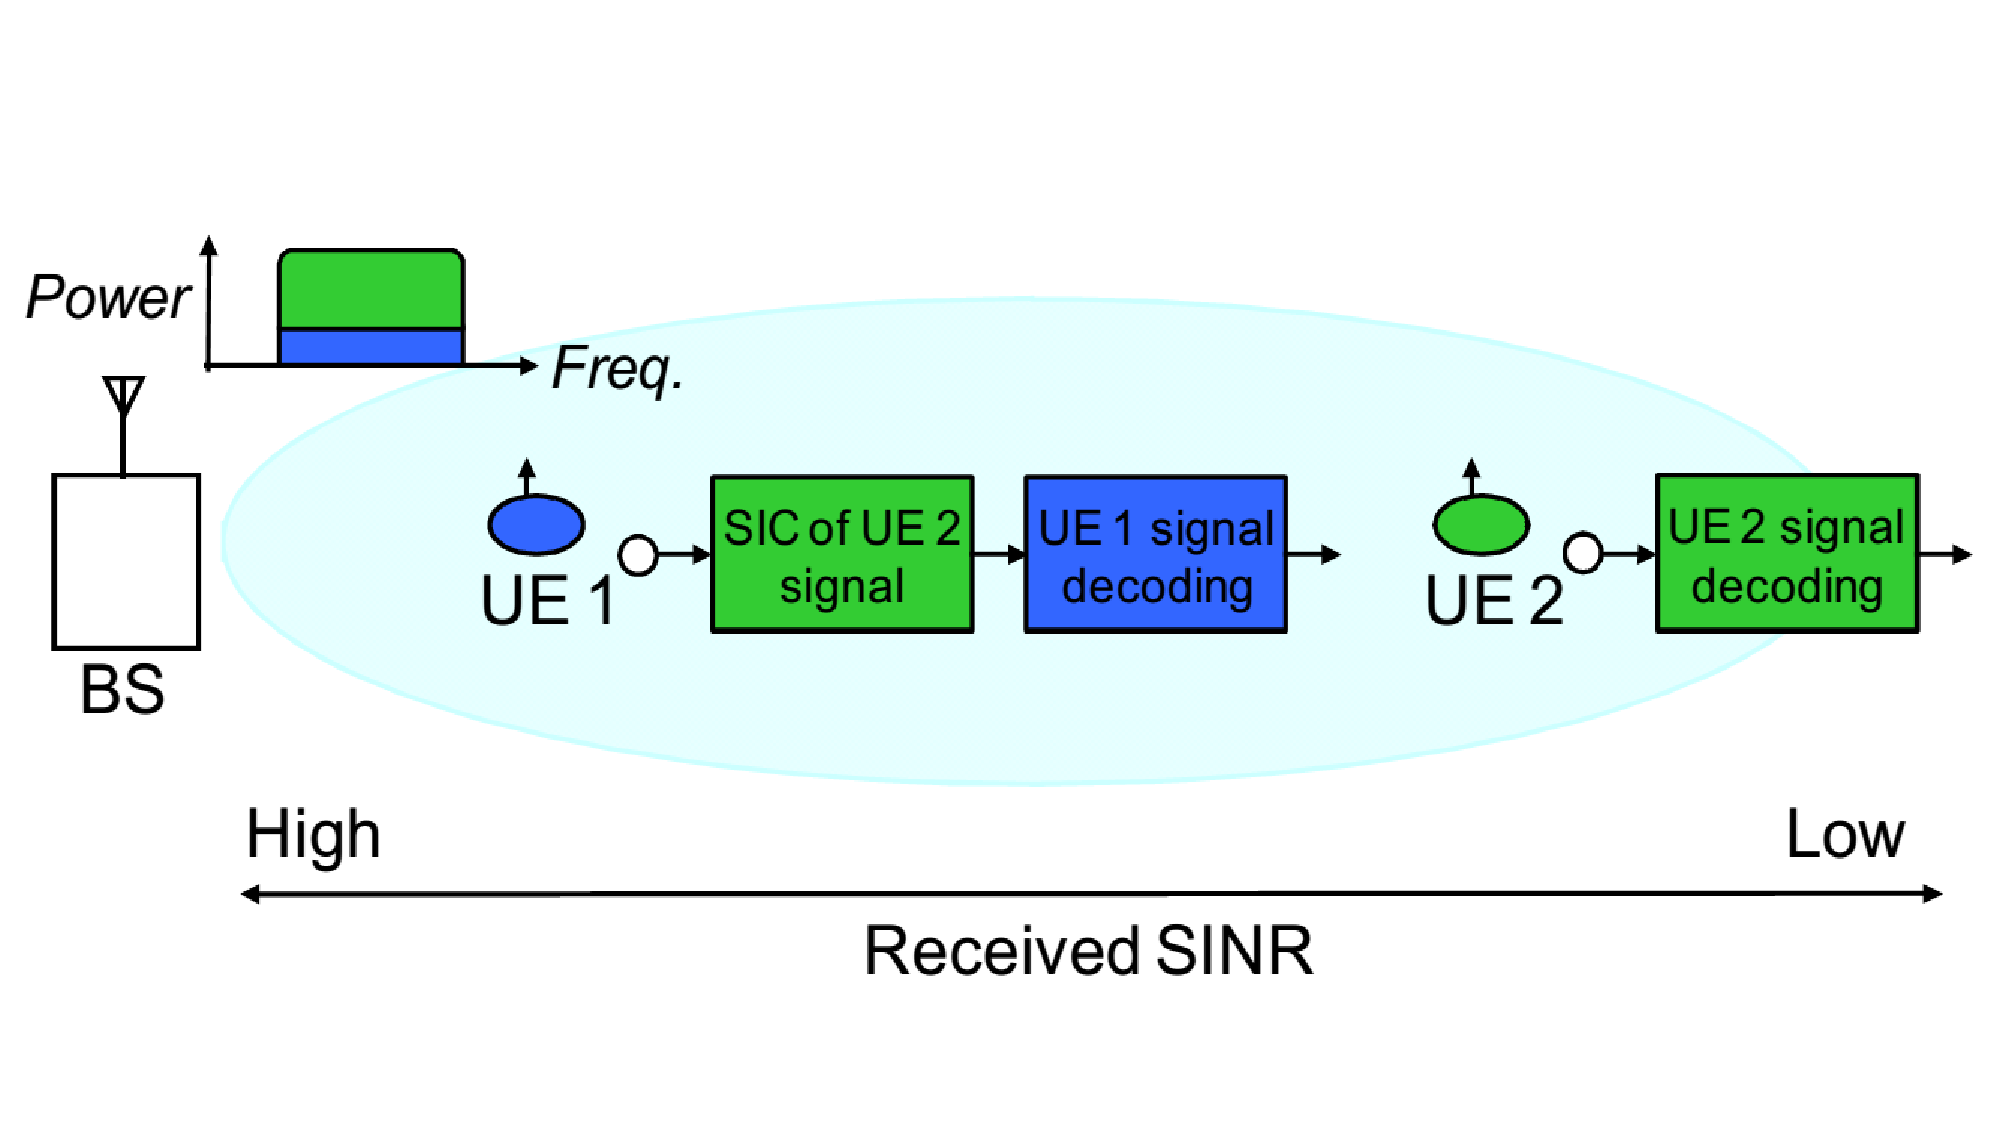
\includegraphics[width=1\columnwidth ,angle=0]{figure/NOMA_shannon}
\caption{Two-user SIC in the downlink}
\label{fig_NOMA_shannon}
\end{center}
\end{figure}
%

%\subsection{Analysis starting from Shannon capacity}
%\label{sec_phy_shannon}

To allow non-orthogonal access from multiple users over the same radio resource, successive interference cancellation (SIC) 
or superposition coding has been popularly considered in the literature~\cite{cite_docomo1,cite_docomo2,cite_docomo3}.
%From our survey in~\cite{cite_docomo1,cite_docomo2,cite_docomo3}, the research about NOMA with SIC in Japan uses Shannon capacity to analyze. 
To understand how SIC works, take the two-user downlink communication in Fig.~\ref{fig_NOMA_shannon} as an example. The transmitted signal from the base station is a linear combination of the signals intended for UE1 and UE2. To decode individual signals, SIC needs to be performed at
each receiving UE. 
%In the NOMA downlink, the SIC process is implemented at the UE receiver. 
The optimal order for decoding is the order of the increasing channel gain normalized by the noise and inter-cell interference power. 
Assuming that the channel gain of UE1 is better than UE2, if UE2 can decode its signal, then UE1 must also be able to decode the UE2 signal.
Therefore, as shown in Fig.~\ref{fig_NOMA_shannon}, UE1 first decodes the signal of UE2 and then decodes its signal after the decoded
UE2 signal has been subtracted. 
%has to decode UE2's signal before decoding its signal, which is the concept of interference cancellation. 
For UE2, it can simply go ahead and decode its own signal without decoding the signal for UE1 first.
%However, UE2 does not perform interference cancellation. 
The case for SIC by $K$ UEs can be performed similarly, and ideally for any UE
the optimal decoding is to remove the interference coming from UEs with worse channel gains.
%, so (\ref{eq_sic_shannon}) is ideal interference cancellation.
As shown in~\cite{cite_docomo1}, 
the achievable rate $R_b^{\text{(sic)}}(k)$ for UE $k$ in resource $b$ can be represented as follows:
%accessing b-th resource and the k-th user throughput with SIC, , is represented as
\begin{equation}
\label{eq_sic_shannon}
R_b^{\text{(sic)}}(k)=W_b \text{log}_2 \left(1+\frac{|h_{k, b}|^2 P_{k, b}}{\displaystyle\sum^K_{{i=1} \atop {\frac{|h_{k, b}|^2}{N_{k, b}} < \frac{|h_{i, b}|^2}{N_{i, b}}}} |h_{k, b}|^2 P_{i, b} +W_b N_{k, b}} \right),
\end{equation}
where $|h_{i, b}|^2$ is channel gain between UE $i$ and the base station, $W_b$ is the bandwidth of resource $b$, $P_{i, b}$ is the transmission power allocated to UE $i$, and $N_{i, b}$ is the noise and inter-cell interference power for UE $i$.
% 分母中的sum是k沒有錯,指的是到第k-th user的i-th signal


%\subsection{Analysis starting from modulation/PER}
%\label{sec_phy_modulation}

In practice, it might not be possible to achieve perfect interference cancellation.
%Without considering partial interference cancellation and modulation, (\ref{eq_sic_shannon}) is too optimistic to evaluate the performance of NOMA with SIC. 
The authors in~\cite{cite_bell1} have show simulation results for SIC with respect to modulation schemes and SNR difference as given in Fig.~\ref{fig_NOMA_modulation}. All points enclosed in the upper right area of each curve are in the desired operating region with $\text{PER} \leq 10^{-2}.$  
Table~\ref{tb_NOMA_modulation} further shows the relationship between modulation and SNR for three marked points in the figure. We can find that the simulation result does not strictly follow (\ref{eq_sic_shannon}). For example, if the SNR of U1 becomes 8 times (i.e. 9 dB) larger, the modulation of U1 can upgrade from QPSK to 16QAM, which has only 2 times larger capacity. 
%
Fig.~\ref{fig_NOMA_modulation} motivates our further investigation on the practical performance of SIC for MAC layer design.
%Therefore, (\ref{eq_sic_shannon}) should be modified and we will analyze how to construct SNR-modulation model and equation in the future works.


\begin{figure}[t]
\begin{center}
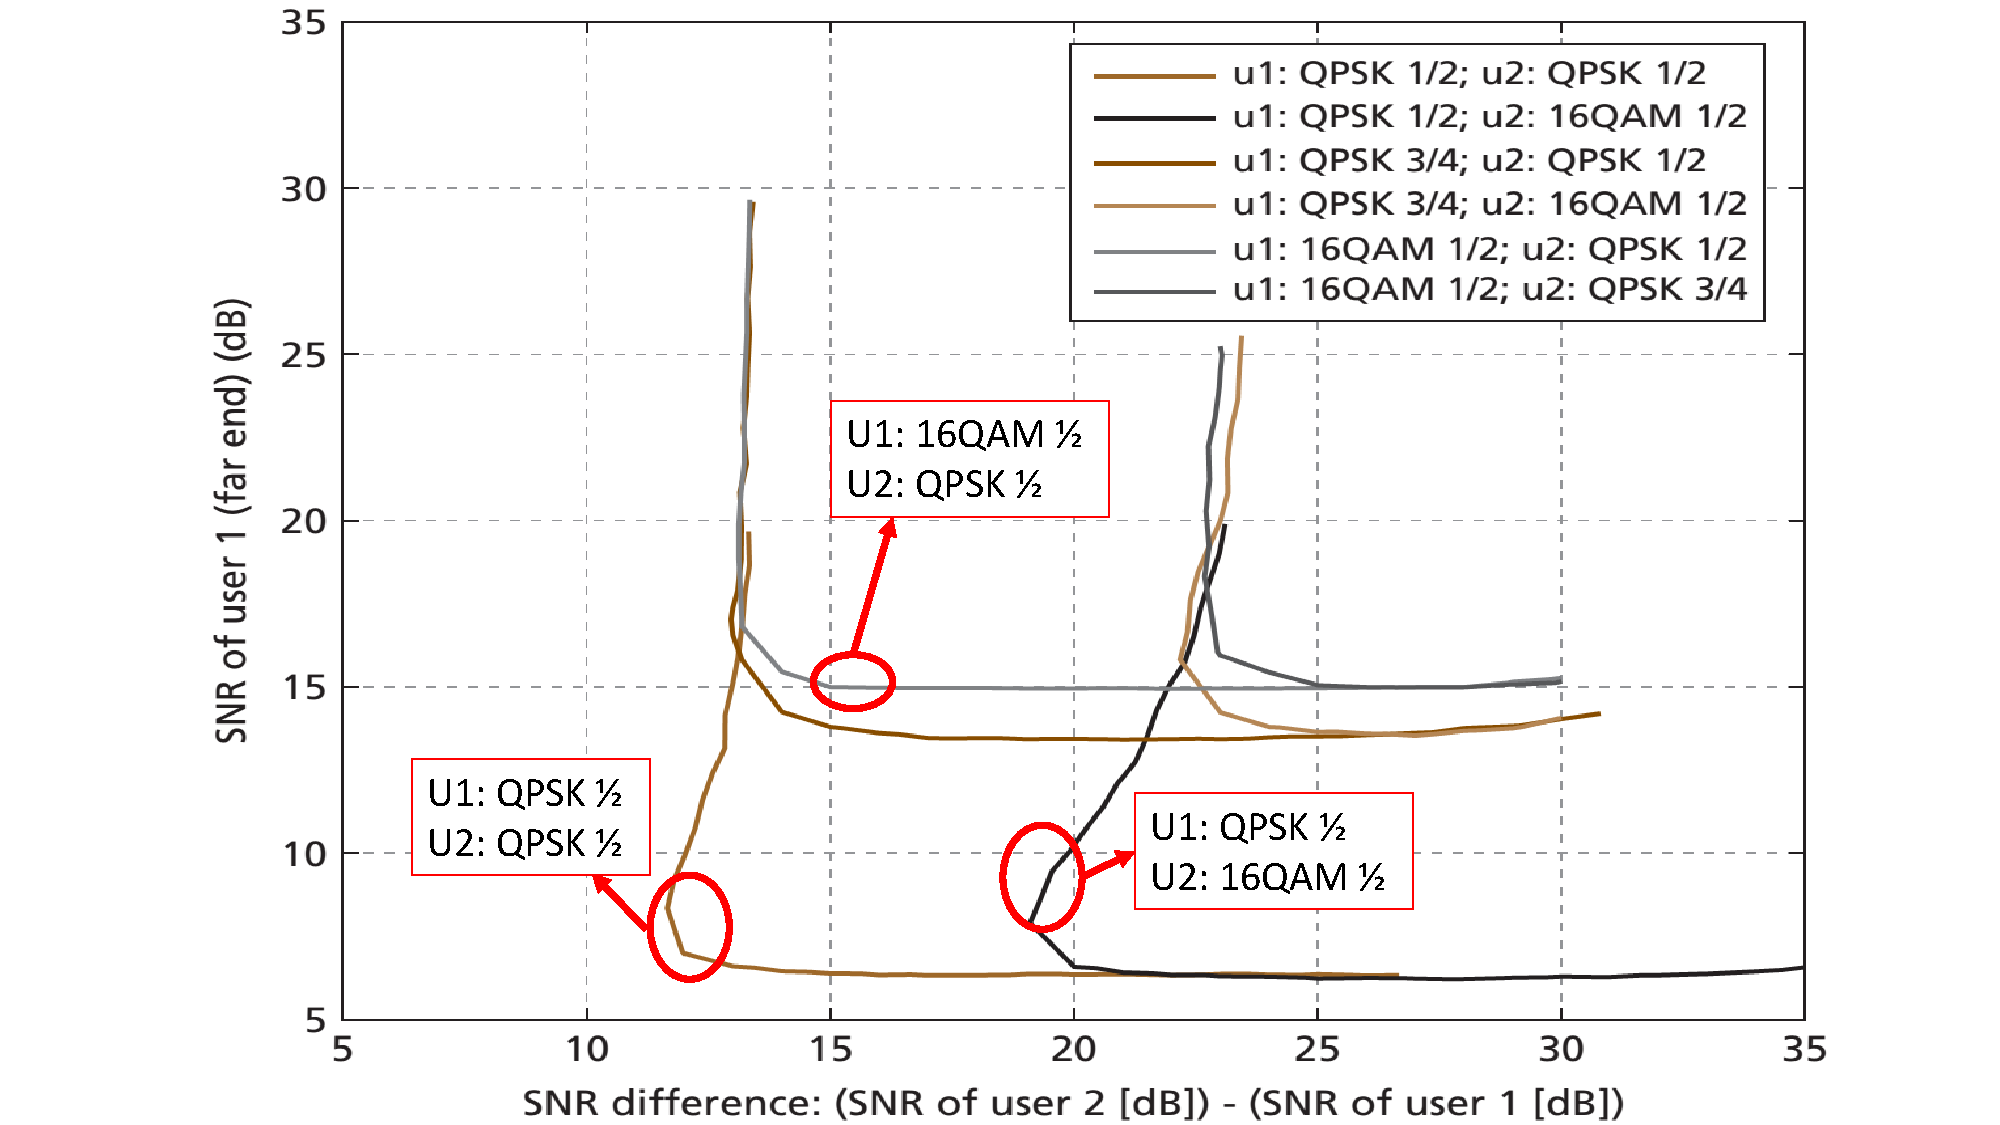
\includegraphics[width=1\columnwidth ,angle=0]{figure/NOMA_modulation}
\caption{Modulation and PER vs. SNR difference}
\label{fig_NOMA_modulation}
\end{center}
\end{figure}
%

\begin{table}[t]
\caption{Modulation curve in Fig.~\ref{fig_NOMA_modulation}}
    \begin{tabular}{| l | l | l | l |}
    \hline
    U1 Modulation & U2 Modulation & SNR of U1 & SNR Difference \\ \hline
    QPSK 1/2       & QPSK 1/2       & 6-15           & 12-20                  \\ \hline
    QPSK 1/2       & 16QAM 1/2     & 6-15           &  $\geq$ 20                     \\ \hline
    16QAM 1/2     & QPSK 1/2       & $\geq$15            & 12-20                   \\ \hline
    \end{tabular}
\label{tb_NOMA_modulation}
\end{table}

